\chapter{Implementacija i korisničko sučelje}
		
		
		\section{Korištene tehnologije i alati}
		
		\textit{Pri izradi ove aplikacije koristili smo brojne alate. To su redom: }\\
		\textbf{\textit{LaTex}}\\
		\textit{LaTeX je programski jezik za pisanje strukturiranih tekstova i njihov automatski slog i prijelom u dokumente profesionalne kvalitete spremne za tisak. Nadogradnja je makro-jezika TeX Donalda Knutha. Za razliku od programa za obradu teksta s grafičkim sučeljem poput Microsoft Word ili LibreOffice Writer koji prikazuju tekst onako kako će izgledati u konačnom dokumentu, dokumenti se za LaTeX pišu kao običan tekst s dodanom semantičkom strukturom. Ovime se, posebno u većim dokumentima, postiže usredotečenost na sadržaj umjesto na izgled, ujednačenost izgleda, te brži i stabilniji rad.}\\
		\textbf{\textit{GitLab}}\\
		\textit{GitLab je internet stranica koja korisnicima omlakšava grupne radove na zajedničkim kodovima. Lakoću korištenja GitLaba osigurava mogućnost izrade više različitih brancheva u kojima jedan ili više korisnika mogu odvojeno od ostatka tima raditi svoj dio projekta. GitLab je jedna od najkorištenijih web stranica u svom području}\\
		\textbf{\textit{Docker}}\\
		\textit{Docker je primjer PaaS (platform as a service) koji korisnicima omogućava virtualizaciju softvera u vidu kontejnera. Docker omogućava korisnicima da isti softver mogu pokrenuti na više operacijskih sustava, što znatno olakšava korištenje aplikacije}\\
		\textbf{\textit{PostgreSQL}}\\
		\textit{PostgreSQL (poznat i kao Postgres ili pgsql) je besplatan sustav za upravljanje bazama podataka otvorenog koda. Sustav poštuje ACID principe pri izvođenju transakcija. PostgreSQL je jedan od najkorištenijih sustava za upravljanje bazama podataka}\\
		\textbf{\textit{Vue.js}}\\
		\textit{Vue.js je 'open source' MVC frontend JavaScript framework za izradu aplikacija. Vue koristi sintaksu baziranu na HTML-u.}\\
	   \eject 
			
			
			\eject 
		
	
		\section{Ispitivanje programskog rješenja}
			
			\textbf{\textit{dio 2. revizije}}\\
			
			 \textit{U ovom poglavlju je potrebno opisati provedbu ispitivanja implementiranih funkcionalnosti na razini komponenti i na razini cijelog sustava s prikazom odabranih ispitnih slučajeva. Studenti trebaju ispitati temeljnu funkcionalnost i rubne uvjete.}
	
			
			\subsection{Ispitivanje komponenti}
			\textit{Potrebno je provesti ispitivanje jedinica (engl. unit testing) nad razredima koji implementiraju temeljne funkcionalnosti. Razraditi \textbf{minimalno 6 ispitnih slučajeva} u kojima će se ispitati redovni slučajevi, rubni uvjeti te izazivanje pogreške (engl. exception throwing). Poželjno je stvoriti i ispitni slučaj koji koristi funkcionalnosti koje nisu implementirane. Potrebno je priložiti izvorni kôd svih ispitnih slučajeva te prikaz rezultata izvođenja ispita u razvojnom okruženju (prolaz/pad ispita). }
			
			
			
			\subsection{Ispitivanje sustava}
			
			\textbf{\textit{Ispitni slučaj 1: provjera ispravnosti logina}}\\
			\textbf{\textit{Ulaz:}}\\
			
			 \textit{1. Korisnik se ulogira u sustav kao user}\\
			 \textit{2. Korisnik se ulogira u sustav kao trainer}\\
			 \textit{3. Korisnik se ulogira u sustav kao club owner}\\
			 \textit{4. Korisnik se ulogira u sustav kao admin}\\
			 \textit{5. Korisnik, pri pokušaju logina, ostavi mjesto za username prazno}\\

			 \textbf{\textit{Očekivani rezultat:}}\\

			 \textit{1. Sustav korisnika prebacuje na početnu stranicu - login je prošao uspješno}\\
			 \textit{2. Sustav korisnika prebacuje na početnu stranicu - login je prošao uspješno}\\
			 \textit{3. Sustav korisnika prebacuje na početnu stranicu - login je prošao uspješno}\\
			 \textit{4. Sustav korisnika prebacuje na početnu stranicu - login je prošao uspješno}\\
			 \textit{5. Sustav javlja error i vraća korisnika na stranicu /auth}\\

			 \textbf{\textit{Rezultat:}}\\
			 \textit{Svi testovi su zadovoljeni, aplikacija je prošla test!}\\

			 \textbf{\textit{Ispitni slučaj 2: provjera ispravnosti registracije}}\\
			 \textbf{\textit{Ulaz:}}\\
			 
			  \textit{1. Korisnik se pokušava registrirati u sustav sa ispravnim podacima}\\
			  \textit{2. Korisnik se pokušava registrirati u sustav sa pogrešno unesenim mailom}\\
 
			  \textbf{\textit{Očekivani rezultat:}}\\
 
			  \textit{1. Sustav korisnika prebacuje na početnu stranicu - registracija je prošla uspješno!}\\
			  \textit{2. Sustav javlja error i vraća korisnika na stranicu /auth}\\
 
			  \textbf{\textit{Rezultat:}}\\
			  \textit{Svi testovi su zadovoljeni, aplikacija je prošla test!}\\

			  \textbf{\textit{Ispitni slučaj 3: provjera ispravnosti kreacije kluba}}\\
             \textbf{\textit{Ulaz:}}\\
             
              \textit{1. Korisnik se pokušava registrirati u sustav sa ispravnim podacima}\\
              \textit{2. Korisnik se pokušava registrirati u sustav krajnjim datumom prijave koji je u prošlosti}\\
 
              \textbf{\textit{Očekivani rezultat:}}\\
 
              \textit{1. Sustav korisnika prebacuje na početnu stranicu - registracija je prošla uspješno!}\\
              \textit{2. Sustav javlja error i vraća korisnika na stranicu za unos podataka}\\
 
              \textbf{\textit{Rezultat:}}\\
              \textit{Svi testovi su zadovoljeni, aplikacija je prošla test!}\\
			 
			
			\eject 
		
		
		\section{Dijagram razmještaja}
			
			
			 \textit{Na poslužiteljskom računalu nalaze se web poslužitelj i poslužitelj baze podataka. Web poslužitelj ovisi o poslužitelju baze podataka, što je na dijagramu jasno prikazano odgovarajućom strelicom. Klijenti pristupaju web aplikaciji preko web preglednika. Komunikacija između poslužitelja i klijenata se odvija preko HTTP veze.}
			
			 \begin{figure}[H]
				\includegraphics[scale=0.7]{slike/Dijagram_Razmjestaja.png} %veličina slike u odnosu na originalnu datoteku i pozicija slike
				\centering
				\caption{Dijagram razmještaja}
				\label{fig:razmjestaj}
			\end{figure}


			\eject 
		
		\section{Upute za puštanje u pogon}

 Izvorni kod svih komponenti aplikacije potrebno je postaviti na „GitLab“ platformu jer će se koristiti pri izgradnji kontejnera potrebnih za puštanje aplikacije u pogon. Izvorni kod naše aplikacije dostupan je na adresi \url{https://gitlab.com/programtvogkompjutera1/ples}. 

Deployment izvodimo koristeći „Render“ platformu u oblaku (platform-as-a-service provider) koja nudi infrastrukturu puštanja aplikacije u pogon u kodu. 
		\begin{figure}[H]
			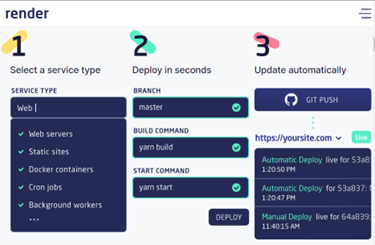
\includegraphics[scale=1.0]{slike/render.PNG} %veličina slike u odnosu na originalnu datoteku i pozicija slike
			\centering
			\caption{Render platfroma}
			\label{fig:render}
		\end{figure}
Prije prijave na „Render“ platformu i kreiranja poveznice prema našem repozitoriju, u korijenskoj mapi izvornog koda potrebno je kreirati "render.yaml" datoteku. Ta datoteka predstavlja „Blueprint spec“ - konfiguraciju potrebnu za izvođenje i puštanje aplikacije u pogon na „Render“ platformi.

Unutar datoteke potrebno je definirati tri servisa koji predstavljaju komponente aplikacije – „server“, „client“ i „db“.  Svaki servis, osim servisa vezanog u „PostrgeSQL“ bazu, mora sadržavati svojstva "type", "name" i "env". 

Servis vezan uz „PostrgeSQL“ bazu mora sadržavati samo svojstvo "name", a informacije za njegovo izvođenje dostupne su kroz već gotovi i dostupan servis „Render“ platforme. 
\begin{figure}[H]
			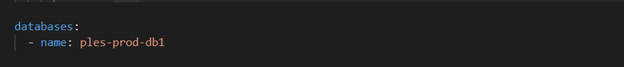
\includegraphics[scale=0.9]{slike/Slika2.PNG} %veličina slike u odnosu na originalnu datoteku i pozicija slike
			\centering
			\caption{Servis baze podataka}
			\label{fig:dbServis}
		\end{figure}

Kod preostalih dvaju servisa - jednog za "frontend", jednog za "backend" navedena svojstva postavljamo kako je prikazano na slikama \ref{fig:ServerServis} i \ref{fig:ClientServis}:

\begin{figure}[H]
			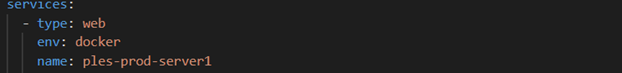
\includegraphics[scale=0.9]{slike/Slika3.PNG} %veličina slike u odnosu na originalnu datoteku i pozicija slike
			\centering
			\caption{Servis servera}
			\label{fig:ServerServis}
		\end{figure}

\begin{figure}[H]
			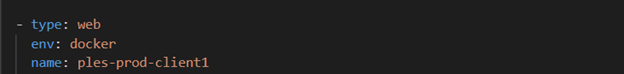
\includegraphics[scale=0.9]{slike/Slika4.PNG} %veličina slike u odnosu na originalnu datoteku i pozicija slike
			\centering
			\caption{Servis klijenta}
			\label{fig:ClientServis}
		\end{figure}

Svojstvo „env“, koje predstavlja okruženje izvođenja, potrebno je postaviti na „Docker“ čime definiramo izgradnju naše aplikacije kroz „Docker“ kontejnere.
Svaki definirani servis zapravo predstavlja informacije o „Docker image“ datotekama. Sadržaj tih datoteka uključuje kod komponenti, alate sustava, biblioteke i sve ostale postavke potrebne za izgradnju kontejnera potrebnih za izvođenje aplikacije.

Svaka „Docker image“ datoteka kreirana je koristeći skup naredbi definiran u datotekama naziva „Dockerfile" koje se nalaze u izvornom kodu aplikacije (jedna za „server“ - slika \ref{fig:ServerDoc}, jedna za „client“- slika \ref{fig:ClientDoc}). „Render“ iz tih datoteka dohvaća „startCommand“ svojstvo kojim se pokreće pojedini kontejner. 
\begin{figure}[H]
			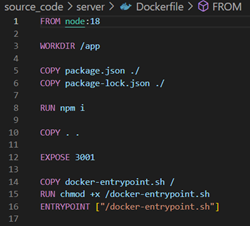
\includegraphics[scale=0.9]{slike/Slika5.PNG} %veličina slike u odnosu na originalnu datoteku i pozicija slike
			\centering
			\caption{Dockerfile server}
			\label{fig:ServerDoc}
			
		\end{figure}
\begin{figure}[H]
			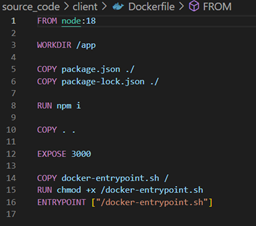
\includegraphics[scale=0.9]{slike/Slika6.PNG} %veličina slike u odnosu na originalnu datoteku i pozicija slike
			\centering
			\caption{Dockerfile klijent}
			\label{fig:ClientDoc}
		\end{figure}
Svojstvo „repo" kod oba servisa postavljamo na putanju na kojoj je dostupan repozitorij sa izvornim kodom aplikacije. Ovo svojstvo govori „Render“ platformi gdje se nalazi izvorni kod aplikacije koja će biti puštena u pogon.

Svojstvo „branch" postavljamo na „master" granu repozitorija definiranog pod "repo", dok svojstvom „rootDir" svakom servisu definiramo korijensku mapu unutar repozitorija gdje se nalazi sav kod potreban za izgradnju i izvođenje tog pojedinog servisa aplikacije. 

Svojstvo „buildFilter" potrebno je za svaki servis postaviti na uzorak putanje koji predstavlja lokacije datoteka unutar repozitorija čije bi izmjene na „master“ grani  trebale uzrokovati ponovnu izgradnju pojedinog servisa (redeployment).
\begin{figure}[H]
			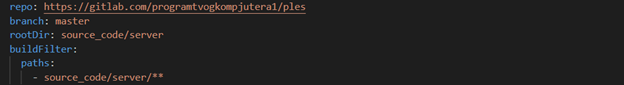
\includegraphics[scale=0.9]{slike/Slika7.PNG} %veličina slike u odnosu na originalnu datoteku i pozicija slike
			\centering
			\caption{Direkoriji servera}
			\label{fig:ServerRepo}
		\end{figure}
\begin{figure}[H]
			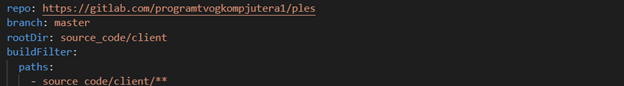
\includegraphics[scale=0.9]{slike/Slika8.PNG} %veličina slike u odnosu na originalnu datoteku i pozicija slike
			\centering
			\caption{Direktoriji klijenta}
			\label{fig:ClientRepo}
		\end{figure}

Ova svojstva zapravo omogućuju automatski redeployment samo onog dijela aplikacije kod kojeg su na „master“ grani uvedene nove promjene u odnosu na zadnji deploy.  

Uz dosad navedena svojstva, još je potrebno definirati varijable okruženja. 

„Render“ nudi mogućnost ovisnosti varijabli okruženja jednog servisa o svojstvima već gotovih „Render“ servisa. Varijable okruženja koje koristimo za spajanje „backend“ servisa na bazu podataka dohvaćamo preko definiranih svojstava „Render“ gotovog servisa za „PostgreSQL“ bazu podataka. Ostale varijable okruženja, koje ne bi smjele biti dostupne svima, stavljamo direktno na „Render“ platformu prije spremanja promjena.
\begin{figure}[H]
			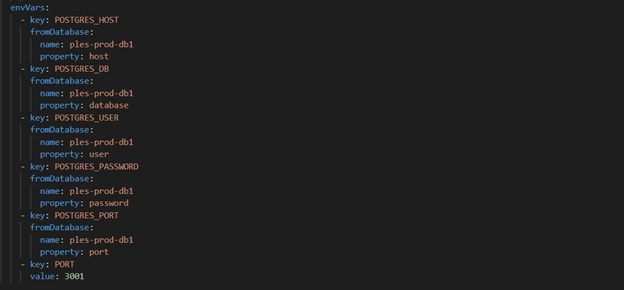
\includegraphics[scale=0.9]{slike/Slika9.PNG} %veličina slike u odnosu na originalnu datoteku i pozicija slike
			\centering
			\caption{Varijable okruženja za spajanje na bazu podataka}
			\label{fig:EnvDb}
		\end{figure}

Za korištenje već navedene platforme, prvo je potrebno napraviti račun te se prijaviti na adresi \url{https://dashboard.render.com/}. Nakon izrade računa u navigaciji „Render“ web aplikacije potrebno je odabrati „Blueprints" te "New Blueprint Instance" - u ovom koraku potrebno je izabrati repozitorij i granu na kojoj se nalazi naš izvorni kod aplikacije u čijem se korijenskom direktoriju nalazi gore opisana "render.yaml" datoteka. („Render“ platforma nudi unošenje podataka o vlastitom računu na „GitLab“ platformi i povezivanje s dostupnim repozitorijima). 

Nakon spremanja promjena, „Render“ web aplikacija povezana je s repozitorijem u kojem se nalazi izvorni kod aplikacije sa „render.yaml“ - slika \ref{fig:yaml} datotekom. „Render“ dohvaća i čita sadržaj te datoteke te na temelju definirane konfiguracije pušta aplikaciju u pogon.
\begin{figure}[H]
			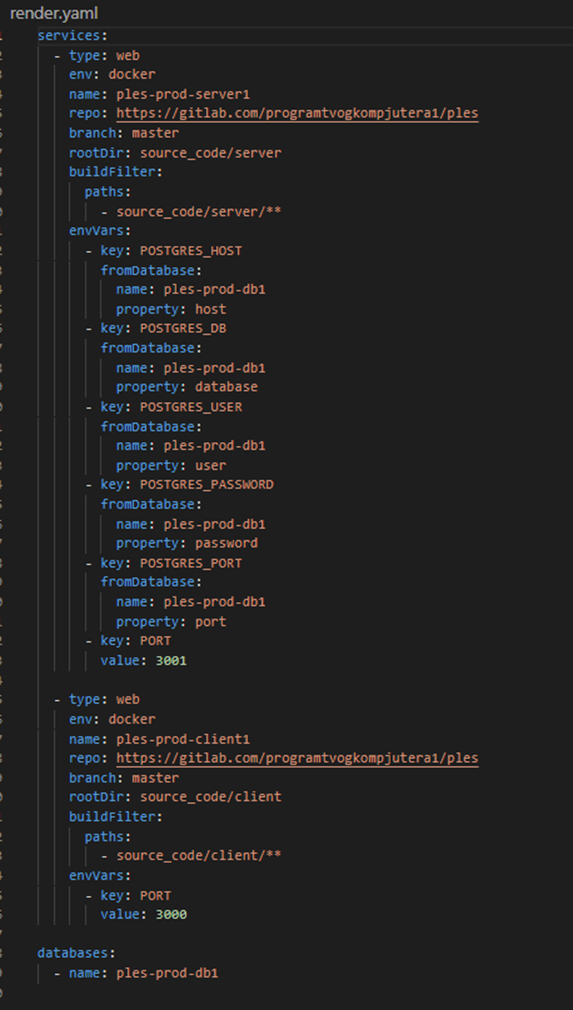
\includegraphics[scale=0.7]{slike/Slika10.PNG} %veličina slike u odnosu na originalnu datoteku i pozicija slike
			\centering
			\caption{Prikaz cijele "render.yaml" datoteke}
			\label{fig:yaml}
		\end{figure}

Aplikacija puštena u pogon se može pokrenuti na adresi \url{https://ples-prod-client1-goj4.onrender.com/}.

			\eject 
			
			
			\eject 